169. \begin{figure}[ht!]
\center{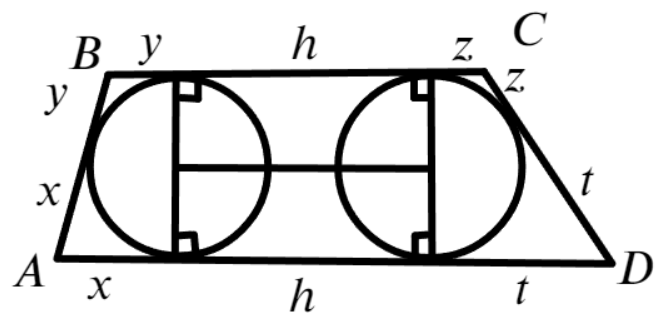
\includegraphics[scale=0.35]{g9-169.png}}
\end{figure}\\
Отметим на картинке равные отрезки до точек касания и составим систему уравнений:\\ $\begin{cases}x+y=4,\\ z+t=5,\\ y+h+z=15,\\ x+h+t=20.\end{cases}$ Сложим два последних уравнения и вычтем из них два первых: $y+h+z+x+h+t-x-y-z-t=2h=15+20-4-5=26,$ откуда $h=26:2=13.$\\
